
%(BEGIN_QUESTION)
% Copyright 2015, Tony R. Kuphaldt, released under the Creative Commons Attribution License (v 1.0)
% This means you may do almost anything with this work of mine, so long as you give me proper credit

Suppose a time-overcurrent (51) relay is configured for a pickup current setting of 3.5 amps and a time-dial setting of 6.  The following curves describe this relay's trip-time characteristics:

$$\includegraphics[width=15.5cm]{i02875x01.eps}$$

First, determine the approximate amount of time it will take for this 51 relay to trip given a constant line current of 1050 amps (assume a CT ratio of 600:5).  Next, determine a new time-dial setting to make the relay trip in approximately 9 seconds at this same amount of line current.

\underbar{file i02875}
%(END_QUESTION)





%(BEGIN_ANSWER)

A line current of 1050 amps is {\it 2.5 times} the pickup current value, which falls directly on one of the vertical lines in this graph.

\vskip 10pt

Trip time at 1050 amps $\approx$ \underbar{\bf 3.5} seconds 

\vskip 10pt

Time dial setting for trip time of 9 seconds = \underbar{\bf 15} 

%(END_ANSWER)





%(BEGIN_NOTES)

{\bf This question is intended for exams only and not worksheets!}.

%(END_NOTES)


